\section{Peeling along monochromatic walls}
\label{sec:peeling}

Throughout Sections~\ref{sec:peeling}--\ref{sec:loops}, fix
$1\le q<4$ and write $4<\kappa=\kappa(q)\le6$.
We now construct a joint exploration toward interior targets.  The boundary
conditions in this construction are part of the proof: its initial law is
the wired FK law in a square, and its final application will be to the
free infinite-volume law of Subsection~\ref{intro:collections}.

\subsection{Actual walls, caps, and the exact exploration law}
\label{peel:construction}

Begin with a nearest-neighbor square whose boundary primal edges are
deterministically open.  Attach to the inward side of each boundary edge
the corresponding half-tile.  Its two ports are paired around its dual
corner; this triangle contains no random switch.  More generally, a
\emph{homogeneous wall} of color $C\in\{{\sf P},{\sf D}\}$ consists of
actual open $C$-edges and these deterministic triangles on its inward
side.  Actual paths along the wall are allowed.  This distinction from
an abstract boundary identification will be used in every crossing
argument below.

All strands are oriented with primal on the left.  To start an
exploration in a primal-walled component, remove one wall triangle.
Enter at its earlier port in counterclockwise boundary order; the other
port is the force port.  On a dual wall reverse the boundary order.  The
boundary of an active component, in counterclockwise order, is
\begin{equation}\label{peel:boundary}
 P_WD_W,\qquad [D_W,D_O]_{\sf D},\qquad
 D_OP_O,\qquad [P_O,P_W]_{\sf P}.
\end{equation}
The first and third pieces are tile sides, while the second and fourth
are actual open dual and primal paths with their deterministic inward
triangles.  Either path may have length zero.  Boundary occurrences,
rather than just geometric vertices, specify the accesses in this
description.

Here is the update at the tip side $P_WD_W$.
\begin{enumerate}[label=\textup{(\roman*)}]
\item If the next tile is fresh, reveal its switch.  In the primal-open
case, cut along its open diagonal $P_WP'$, remove the triangle traversed
by the strand, and continue from $P'D_W$ on the two-change side.  The
other half-tile becomes a deterministic wall triangle.
\item If $P'$ is an interior vertex, there is only one active component.
If it is a boundary occurrence, the new diagonal is a proper crosscut
joining the primal arc to itself.  It cuts off a homogeneous primal
pocket.  Retain the component containing the target.  In the pocket,
remove the triangle on the \emph{next counterclockwise old-wall edge}
starting from the hitting occurrence $P'$ and restart there.  For targets
on the two-change side, continue the old strand.
\item For a dual-open switch use the same rule with the colors exchanged
and clockwise order.  If the tip meets a known triangle, remove it and
follow its cap to the other leg.  This shortens the wall instead of
adding an edge.
\end{enumerate}
The rule is understood in the sector seen from the tile.  The opposite
corner of a newly retained wall triangle lies on its indicated side of
the crosscut.  A known triangle has two consecutive boundary sides in
that sector, so clipping it leaves just the other leg.  In particular
one never glues the two banks of a zero-width slit.  Starting from the
square, nonempty completed components are physically Jordan domains:
an update either indents the boundary through a new interior corner,
cuts it by a proper crosscut, or clips consecutive boundary edges.
The same observations apply when a homogeneous wall is opened.  The
only degenerate terminal configurations lie within a bounded number of
tiles of the target.  They cannot occur on a bounded radial horizon
from a macroscopic starting domain.

\begin{lemma}[Exact pocket law]\label{peel:factorization}
Conditionally on any finite exploration history, the unqueried switches
in its remaining components have the positive cap laws described by
their boundaries.  Distinct components are conditionally independent.
Before two targets split into distinct components their explorations
are identical.  A strand between successive pocket switches is a
portion of one original closed loop.
\end{lemma}

\begin{proof}
At a cut, every matching connection is either the consumed switch pair
or a local cap on one of its sides.  Consequently the factors
$q^{\ell/2}$ for unstarted loops, and the factor for eventually closing
the current strand, have no remaining dependence involving both sides
of the cut.  Their product therefore factors over the components.  A
two-change component has one strand between its ports; closing these
ports outside gives its marginal cap law.  The deterministic triangles
implement exactly those identifications.  No random switch is hidden
in such a triangle.

Until a switch into a homogeneous pocket, every traversed pair belongs
to the loop through the originally opened cap.  At a pocket switch
that loop remains on the other side of the actual open diagonal.
The new cap is on a loop not yet traced in the retained pocket.  This
also proves the last assertion.  For finitely many targets keep the
cut-off components, including their boundary states, and process active
branches in a fixed priority order.  The factorization gives the claimed
conditional independence before taking any limit.
\end{proof}


\subsection{Radial clocks and forcepoint resets}
\label{peel:radial}

For an interior target $z$ let
\[
 t=\log\frac{\operatorname{crad}(U_0,z)}
                    {\operatorname{crad}(U_t,z)},
 \qquad \Phi_t:U_t\longrightarrow\mathbb D,
 \quad \Phi_t(z)=0,
\]
where the argument of $\Phi_t'(z)$ is fixed.  On $t\le T$, Koebe's
theorem supplies a ball about $z$ of radius bounded below in terms of
$T$ and the initial conformal radius.  The chart modulus of
Section~\ref{sec:movingtests} therefore applies uniformly to connected
short paths and to their boundary accesses.

Let $e^{iW_t}$ be the tip and $e^{iO_t}$ the force access.  Choose lifts
so that
\begin{equation}\label{peel:angle}
 \theta_t=O_t-W_t\in[0,2\pi]
\end{equation}
is the angle of the counterclockwise dual boundary arc.  The force
access is at the wall-color endpoint of the force side chosen at the
last opening: after a primal opening this is $P_O$, approached beside
the interior of the side.

We use the following interpolation, which fixes the behavior at
collisions.  Move along the small tip side to the near endpoint of the
new diagonal, grow the diagonal as a slit, and, on the retained
two-change side, grow the other leg of the traversed triangle to clip
it.  Move along the resulting boundary leg to the new port.  For a
known triangle grow its other leg across to clip it.  Boundary motion
itself has zero growing time.  When the slit makes a pocket crosscut,
the force access collapses to the tip: $\theta=0$ in a primal pocket
and $\theta=2\pi$ in a dual pocket.  At a primal restart, move $O$
counterclockwise \emph{ahead}, to the far endpoint of the next edge,
and remove that edge's triangle by growing its two legs in wall order.
Then continue with $W$ at the new start.  Reverse both directions at
a dual restart.  Triangle removals on separated sides of a common
crosscut may subsequently be processed separately.

These updates have disjoint growing-time interiors and produce
exactly the designated target components.  They differ from the medial
strand, including its reset connectors, only inside a bounded number
of adjacent tiles in the accessed sectors.  The chart modulus implies
that all boundary-angle jumps vanish uniformly on bounded horizons.
The capacities of individual updates also vanish: their cuts are
chart-small, and kernel convergence preserves the basepoint component.
The total angular oscillation within one update vanishes as well.
Indeed its cut is in a vanishing sector of its starting chart; the
normalized new maps converge to the old map on compact interior sets
and, by reflection, on closed boundary arcs away from that sector.
The new tip is in that sector, while a force access is either regular
or belongs to the same collapsing sector.

Between the designated resets, the radial boundary equation is
\begin{equation}\label{peel:force-ode}
 dO_t=\cot(\theta_t/2)\,dt.
\end{equation}
If its endpoint is hit but the force side is retained, continue using
the access beside that side.  Convergence in the retained sector,
which can be checked by truncating the access with short circular
gates, gives the same one-sided equation on the next slit.  Its
improper integral at a collision is finite: near the collision the
motion has one sign and the force access has a finite angular limit.
No additional jump of $O$ is introduced.  These conventions also apply
when the end of the newly opened triangle is reached.  Stops at
completed updates suffice in what follows; allowing the switch of a
just-started update changes nothing in the limit.

\subsection{Crossings in the moving charts}
\label{peel:crossings}

We need actual paths reaching the explored wall, including where that
wall is irregular.  The following form specifies both the geometry and
the information retained after a crossing is found.

\begin{lemma}[Wall crossings and screening]\label{peel:wall-rsw}
Fix a buffered corridor of bounded aspect in a normalized disk chart.
Its terminal wall intervals lie strictly inside designated homogeneous
arcs; one terminal interval may instead be an interior bar.  After the
mesh limit at this fixed scale, an actual crossing of either prescribed
color $X$ has conditional probability bounded below, uniformly in the
exploration history and its boundary partitions.  At an $X$-wall it
reaches an actual wall vertex.  At an opposite-color wall it reaches
the $X$-corner of an inward wall triangle.  In the latter case a segment
inside that triangle, ending at the midpoint of its base, completes
the crossing to a screen and meets an actual $X$-path only at its
starting corner.

The two-sided bounded-density collar comparison of
Section~\ref{sec:preliminaries} holds for such buffered chart collars
on a homogeneous wall, with a bounded number of through-wire blocks.
\end{lemma}

\begin{proof}
We explain the reduction to a simple square-lattice quad, so that the
up-to-boundary crossing theorem applies with its exact hypotheses.
For the color $X$, retain the edge-connected component around the
basepoint of square faces whose centers have $\ell^\infty$ distance
more than $k\delta$ from the planar complement; a fixed $k=20$
suffices.  The failing faces are edge-connected, as one sees by
rasterizing a thickened path in the connected complement, including
slit banks.  Other components of passing faces are assigned to the
exterior.  Both face families are then edge-connected.  Alternating
interior and exterior faces at a self-touch vertex would separate one
of these families, so the retained polygon has a simple boundary.
It lies in unqueried territory and eventually contains every compact
chart core.

An incident failing face on its perimeter can be followed, through
$O(k)$ adjacent failing faces, to the first wall contact.  Thus every
perimeter point has a short exterior access to the actual wall.  The
chart modulus implies that the perimeter approaches the unit circle
uniformly and that its separated accesses have the correct cyclic
order.  The winding about the basepoint fixes that order globally.

Approximate the two longitudinal sides of the desired corridor by
simple $X$-lattice crosscuts inside this polygon.  First approximate
their compact interior portions with positive clearance; then append
terminal paths in disjoint chart neighborhoods, stopping at the first
perimeter contact.  Grid shadowing and loop erasure preserve the chart
margins, since each short connected error is chart-small.  Together
with the appropriate perimeter intervals these crosscuts bound a
simple lattice quad.  The transverse margins and angular order bound
its extremal distance by a constant depending only on the buffered
corridor.

This last bound can be made directly in discrete extremal length.
Thicken vertex weights over balls of a few mesh steps, with density
scaled by $\delta^{-1}$.  Each member of a fixed transverse family of
longitudinal chart paths shadows an edge path in the quad, cropped to
the two terminal sides.  Grouping successive connected pieces of
displacement $\delta$ charges only boundedly many nearby vertices.
The shadowed length is therefore bounded by a constant times its
density integral; the squared area integral is bounded by a constant
times the sum of squared vertex weights.  The fixed chart family gives
the asserted extremal-distance bound.

Theorem~1.2 of \citet{DMT2021Fractal} now gives a positive crossing
probability for the simple quad at $p_q$, for $1\le q<4$, with arbitrary
boundary partition.  Equivalently, use the free law as the lower
comparison.  Do not query edges running along its terminal perimeter
sides.  From a reached vertex, an outward failing-face chain gives
$O(k)$ available $X$-edges toward the intended wall.  The extension
uses only those unqueried terminal-side edges and edges outside the
quad.  Finite energy gives a uniform positive conditional cost.  Stop
at the first wall contact; if an opposite-color wall blocks the next
step, the current vertex is already the $X$-corner of its triangle.
This proves the crossing assertion, including its endpoint convention.
Circuits and interior connections with strict margins follow by
ordinary box-crossing and gluing.

For the collar statement, find the same-color screen nearest the
unknown-facing side of a deterministic buffered subcollar.  Paths may
be restricted to the strip between the prescribed wall intervals,
pruned at terminal returns, and augmented by ordered spokes to common
endpoints.  Minimizing the region on the unknown side selects a
simple outermost crossing.  Any competing path entering strictly
nearer that side has an open excursion that can replace part of the
selected path and decrease this region.  Hence the selection tests
only on and on that side of the screen.  Its other side retains an
FK law with a boundary partition.

Actual paths of the screen's color must attach to it in order to cross.
An opposite-color path cannot pass it except through the bounded
through-wire blocks; the added segment in a wall triangle creates no
other bypass.  Splitting or merging those blocks changes a weight by
a bounded factor.  The primal and dual screening searches used in the
collar proof of Section~\ref{sec:preliminaries} thus apply without
change to arbitrary-event densities.  All chart margins are fixed
before the mesh limit, as required.
\end{proof}

\subsection{A bound on generations}
\label{peel:generations}

\begin{lemma}[Disjoint passages and reference walls]
\label{peel:passages}
The number of edge-disjoint actual monochromatic cycles surrounding a
fixed macroscopic ball in the initial square, and using no deterministic
initial wall edge, is tight as the mesh tends to zero.  Along finitely
many target branches with bounded radial horizons, the number of
reference-wall generations defined below is jointly tight.
\end{lemma}

\begin{proof}
Such cycles provide edge-disjoint vertical passages in a fixed-height
middle horizontal band.  By bounded degree and Menger's theorem,
their number is bounded by a fixed multiple of the maximal number of
vertex-disjoint passages.  For primal paths one may add random switches
on the initial wired boundary edges, which does not change the interior
marginal under consideration.  For dual paths use the rectangle of
interior faces.  Thus it suffices to work in an ordinary fixed-aspect
color-lattice rectangle, with its induced positive FK law.

Prune bottom-to-top paths so they do not return to their terminal rows.
Select the leftmost open path, then the leftmost path to its right that
is vertex-disjoint from it, and repeat.  To justify the information
claim, attach noncrossing spokes just below and above the terminal rows
to common endpoints, pad the rectangle sides, and minimize left area.
Another eligible path entering strictly left gives an excursion with
distinct endpoints on the augmented path and permits replacement in
either traversal direction, decreasing left area.  End excursions
through a spoke use only terminal contacts.  The selected path is
therefore determined by its own edges and the edges on its left.  If
$m$ vertex-disjoint passages exist, at least $m-1$ remain to its right,
and the argument iterates.

After a selection $p$, there is a uniformly positive conditional
probability of blocking another disjoint passage.  If $p$ comes within
ten mesh steps of the right wall on some horizontal half-row, force an
opposite-color connection along that row from outside the right wall
to first adjacency to $p$; its finite-energy cost is bounded.  If $p$
already blocks, no forcing is necessary.  Otherwise follow $p$ on its
right through opposite-lattice face centers, joining consecutive ones
inside the right wedges at its vertices.  Erase loops and trim terminal
returns to obtain a simple path $p_*$ between the extreme interior
half-rows.  Those rows are single intervals on the right side because
$p$ was pruned.  With them and the rightmost interior column, $p_*$
bounds a simple opposite-lattice quad of fresh edges.

Horizontal rows give a bounded-extremal-distance family across this
quad: there are order-height disjoint rows, each of length at most
order-width.  Lemma~\ref{peel:wall-rsw}, or directly
\citet[Theorem~1.2]{DMT2021Fractal}, supplies an opposite-open crossing
with uniformly positive probability.  Extend it one step beyond the
right boundary at finite-energy cost.  At its other endpoint, append
a segment in the incident square to a vertex of $p$.  This screen
blocks all actual vertical paths on the right avoiding vertices of
$p$.  Its edges are fresh under the leftmost-path conditioning.
Consequently the successive selections have a geometric tail; blocker
tests need not themselves be exposed when continuing the search.
In particular, if $N$ is their number, then for constants depending
only on $q$ and the fixed rectangle shape,
\begin{equation}\label{peel:passage-tail}
 \mathbb P(N\ge m)\le(1-c)^{m-1},\qquad
 \sup_{\delta}\mathbb E[e^{aN}]<\infty
 \quad\text{for }0<a<-\log(1-c).
\end{equation}
This proves the first assertion, and also gives the corresponding
bound for a strictly bulk rectangle.

A generation begins in a homogeneous $C$-pocket, whose present wall is
its \emph{reference wall}.  Read the $C$-arc from $O$ to $W$ in
counterclockwise order for primal and clockwise order for dual.  It
consists of a prefix of the remaining reference interval followed by
a suffix of actual open edges revealed during this generation.  A
triangle step shortens this path; a fresh diagonal extends it or
returns to an earlier vertex.  At a same-color switch retaining part
of the prefix, the next gap is precisely its first retained reference
edge.  The description is thus preserved, even when the prefix becomes
empty.  These switches take place on the reference wall.

Start a new generation at the first homogeneous pocket whose retained
arc has no reference edge; every opposite-color switch has this
property.  Its wall consists entirely of actual diagonals discovered
since the previous start.  Consumed edges are not reintroduced by
known triangles.  The successive new reference cycles are consequently
edge-disjoint, separately for each color.  They surround the basepoint
ball present up to the fixed horizon.  If a wall walk has repeated
vertices, its winding extracts a surrounding cycle.  The first
assertion bounds the number of generations.  For finitely many
branches sum the bounds, allowing an ancestral generation to be
counted along each of its descendants.
\end{proof}

\subsection{Local chordal tests in a peeled domain}
\label{peel:localtests}

Put $h=1-2\rho$, with $\rho$ as in Section~\ref{sec:exponents}.
At a causal completed state with $\theta$ in a compact subinterval of
$(0,2\pi)$, map the active domain to $\mathbb H$ so that the tip is
$0$, the force access is $\infty$, and the target has imaginary part
one.  The positive real arc is dual-designated.  Stop a short subsequent
segment at fixed driver and chordal-capacity bounds, chosen so the
target remains safely inside and connected to the force access.  There
are no resets on this segment.  Let $g_t$ and $W_t^{\mathbb H}$ be its
chordal map and driver.

\begin{proposition}[Tests away from coincidence]\label{peel:martingales}
For $x>0$ beyond these localization bounds, the quantities
\begin{equation}\label{peel:test}
 M_t(x)=\left(\frac{xg_t'(x)}{g_t(x)-W_t^{\mathbb H}}\right)^h
\end{equation}
satisfy the approximate martingale identities between arbitrary causal
stops on the segment.  Tests may include the entire earlier exploration
history of finitely many targets.  The errors tend to zero after the
mesh limit.  The assertion concerns the averaged identities for this
history law, not a uniform assertion over all deterministic mazes.
\end{proposition}

\begin{proof}
We supply the modifications needed to apply the moving-domain
comparison of Section~\ref{sec:movingtests}.

\paragraph{The test notch.}
Fix first a small chart scale $s>0$.  Cut a notch around $x$, of size
between $s$ and $2s$, with two transverse ends on the old dual wall.
Put a new separate primal wire only on the middle portion of its new
wall, a positive chart distance from those ends, and keep dual
designations on both flanks.  Approximate a regular semicircular or
polygonal notch by openable dual diagonals near its ends and openable
primal diagonals in its strictly interior middle, with transition tile
sides.  The artificial diagonals are deterministic in the modified
experiment.  The result has four changes with the same triangular-cap
convention as before.

This construction is possible in unqueried territory.  Compact
interior parts have ordinary positive-clearance approximations; end
parts shadow dual-grid paths in the prescribed accessed corridors up
to first actual dual-wall contact.  Loop erasure preserves their order
by the chart margins.  We also choose the notch to have controlled
physical terminal tails.  Length-area, applied to a positive-width
family of chart curves, bounds the integral of the inverse-curve tail
lengths below height fraction $\epsilon$ by $O(\sqrt\epsilon)$, since
the physical area is bounded.  Thus a curve can be chosen with tails
vanishing at shrinking height cutoffs.  One may make the height cutoff
decrease slowly with the mesh.  Its retained interior is approximated
with positive one-sided clearance, and the new primal interval stays
at positive physical distance from all previous and locally stopped
trajectory pieces for fixed $s$.

\paragraph{Exact identities and comparison of the histories.}
Sample the notched law conditionally at the start of the segment.
Follow its strand until the localized stop, measuring the stop in the
unnotched geometry.  The strand cannot reach or swallow the notch
data: real and complex Loewner ODE bounds keep its growth away from
that chart neighborhood.  Every locally discarded pocket is
homogeneous and contains neither notch nor force data.

The pairing probability with the two primal wires separate is an
exact martingale.  Identifying the two primal intervals gives the
complementary dual comparison; its law is a bounded tilt depending
only on the pairing.  These identities are taken at completed states.
For additional targets keep reporting geometry and scheduling from
the unnotched cuts until the local stop or an active horizon, without
changing a target assignment near the notch.  Still-shared targets
see this same growth, and separated components have their ordinary
independent laws by Lemma~\ref{peel:factorization}.  If a target clock
freezes, truncate the identity there.

Lemma~\ref{peel:wall-rsw} compares the exterior history laws, for fixed
$s$, by bounded density constants.  To obtain a coupling error tending
to zero as $s\downarrow0$, bracket the exterior primal partitions at
the notch by the extremal partitions, expose actual attachment
clusters in the stronger law, and block them by dual wall-to-wall
paths in successive dyadic chart half-collars.  These lie away from
the old primal wire, so there is no primal wire bypass.  Conditional
success probabilities at each fixed-shape scale are uniform after
the mesh limit.  Only the separate-primal-wire law is needed in this
last coupling, not its pairing tilt.

\paragraph{Rough-domain obstacles.}
For a later stopped notched domain, its four-change rectangle is
nondegenerate for fixed $s$.  The central possible-attachment vertices
and their optimistic color paths are defined exactly as in the
moving-domain argument.  Accessible identifications and deterministic
open adjacencies have short accesses to their assigned wires.
Away from those wires a central attachment begins with an actual
uncertain-edge path to macroscopic distance.  Protected-ball deletion
still has only rim attachments in the relevant components; splitting
a physical vertex weakens these connections.  No notch cap supplies
a shortcut of a color away from that color's electrodes.

Use the initial square, the relevant ancestral and current exploration
pieces, and the notch as obstacles.  First truncate the numbers of
branches and generations, using Lemma~\ref{peel:passages}.  Within
generation $j$, retain excursions reaching depth $r_j$ from the initial
boundary and the earlier-generation obstacles, starting and ending at
much smaller depth $h_j$, or at an active endpoint.  The earlier
obstacles contain its reference wall up to a step-sized error.  Away
from them, each retained leg is jump-free and has actual open paths
of both colors beside one loop portion.  Bulk passage bounds, on a
finite grid of annuli, make the number of these legs and of their
short internal blocks tight.  A trajectory does not retrace a loop
portion: at a switch the old loop remains in the other component.

Choose accuracies backwards through the generations, approximating
each earlier obstacle much better than the descendant depth $h_j$.
Excursion endpoints then attach to earlier routes in protected small
balls, and omitted shallow pieces contribute only $r_j$ to the
Hausdorff error.  Each retained block has a known actual path $\pi$ of
the requested color in a short bulk patch.  The routing and flag
construction of Section~\ref{sec:movingtests} therefore applies on a
finer deterministic grid.  Route the notch on its removed side, with
clearance on compact interior portions, and attach its short terminal
tails in protected balls.  Specifically, fix the two protection radii,
choose still smaller physical tails as above, then approximate the
retained interior by a polygon with one-sided clearance.  At fixed
height cutoffs, normal-family bounds allow all perturbations and
snappings to be chosen from finite lists.  Make earlier obstacle
accuracies smaller afterward, and take mesh errors last.  The resulting
rounded Jordan comparison domain contains every required internal
compact path and has all the limiting complement contacts needed for
kernel convergence; its marked prime data agree in interior charts.

\paragraph{Why the flag cost is the original six-arm cost.}
Use original past switches and actual wire edges for the known legs.
In testing the absence of a short optimistic bridge to $\pi$, allow
even the original unnotched ambient completion.  An actual path leaving
the old domain first hits its designated wall; opposite-color wall
diagonals block it.  The same is true on first contact with a previously
queried edge of its color.  Near the current old wire portions, the
chart modulus excludes a shortcut from a central vertex in a
sufficiently small physical disk.

There are two different locality checks near the notch.  A primal
central path that locally crosses it stays near the old positive
dual-wall patch in the starting chart, far from any old primal contact
or locally grown trajectory; it cannot reach a known primal history
edge there.  For a dual central vertex near a flagged historical
detail, the entire notch is far away in the old chart.  Indeed a
central dual abscissa near the notch must avoid both dual flanks and
their ends, and hence lie in a compact interior chart patch beside the
new primal interval.  That patch has positive physical distance from
the old history and the locally stopped pieces, first by the regular
notch margins and then by the ODE bounds.  Kernel convergence and
analytic continuation away from the local hull give the same assertion
on every shape subsequence.

All these arguments follow connected paths in the old domain until
their first old-wall contact.  Boundary-sector identifications cannot
undo the actual diagonal barriers.  The sector-duality argument thus
produces the original known flags from the two witness arms, and an
actual extra arm produces six alternating arms in the original
ambient switch lattice.

For dual extra arms near flags, the required narrow arm pieces lie
outside the notch and its narrower protecting collar.  The arbitrary-event
collar density comparison transfers their probability, including
the local history, to the original law; the pairing tilt costs another
bounded factor.  For primal extra arms, first compare the stopped
history through the outer collar.  Conditionally on that history the
extra-arm event is increasing in primal edges.  Restore the deleted
notch and wire only the new middle primal vertices locally.  This
dominates the modified law: the dual flanks had imposed no primal
wiring, and their known dual edges had only removed primal choices.
The flagged local arm pieces are physically separated from that new
interior wiring by a vacant bulk collar, containing no earlier history.
The bulk density comparison then transfers their probability to the
original conditional law.

For either color, summing over fine-grid flagged cells consequently
costs a bounded multiple of the original annealed six-arm sum.  Its
decay follows from \citet[Corollary~6.7]{DMT2021Fractal}, after the
collar transfer of Section~\ref{sec:preliminaries}.  Take the grid
scale small after all collar margins, trims, and block cutoffs.
Protected-ball errors, in contrast, are estimated directly
conditionally in the modified law.  The chart and notch may depend on
the segment-start history: at fixed scales their margins and comparison
constants are uniform under the stated normalizations.

\paragraph{The alternating formula and the shrinking notch.}
These checks are the additional inputs required by the upper barrier
comparison of Section~\ref{sec:movingtests}.  Its directed routes have
clearance from central candidates except for the controlled deletions.
The level fibers of the remaining kernel and comparison template agree
outside protected end balls, giving the same shared-graph partition
domination for the abscissa-trimmed quad.  Fix generation cutoffs,
block cutoffs, grids, and all intermediate scales before the mesh
limit.  The preceding averaged bounds make adverse conditional costs
negligible in history probability.  The two color upper bounds and the
pairing tilt therefore identify the stopped conditional pairing
probability with the separate-wire value $g(\chi)$.

Divide its exact martingale identity by the initial formula value,
which is bounded below for fixed $s$.  As $s\downarrow0$, the ratio
tends locally uniformly to \eqref{peel:test}.  To see the conformal
normalization, remove the same small boundary hull near $x$ in the
starting and later chordal charts.  The map between them is analytic
near that hull, with derivative $g_t'(x)$ bounded above and below and
bounded second derivative.  Rescaling the notch gives uniform Jordan
shape convergence, so the flattened prepoint interval widths have
ratio $g_t'(x)(1+o(1))$, while their base positions have ratio
$(g_t(x)-W_t^{\mathbb H})/x$.  The asymptotic
$g(\chi)\sim c\chi^h$ gives \eqref{peel:test}.  Finally use the
vanishing separate-law coupling error to return bounded tests to the
original law.  This order of limits proves the proposition.
\end{proof}

\section{Identification of the joint angular tree}
\label{sec:tree}

\subsection{Interior evolution and an oriented boundary estimate}
\label{tree:tightness}

All assertions in this section are first made for finitely many
fixed deterministic interior targets and bounded radial horizons.
The horizons may subsequently increase.  The small-update estimates
of Subsection~\ref{peel:radial} absorb port ambiguities and the difference
between an interpolated stop and a completed-state stop.

\begin{lemma}[Interior characteristics]\label{tree:interior}
Away from $\theta\in\{0,2\pi\}$, every limiting branch has the local
characteristics
\begin{equation}\label{tree:sde}
 \begin{aligned}
 dW_t&=\sqrt\kappa\,dB_t+
          \frac{6-\kappa}{2}\cot(\theta_t/2)\,dt,\\
 dO_t&=\cot(\theta_t/2)\,dt,\qquad \theta_t=O_t-W_t.
 \end{aligned}
\end{equation}
Here $t$ is that branch's radial clock; the martingale identities hold
relative to the full causal exploration history.
\end{lemma}

\begin{proof}
Use two ordered test points $x$ in Proposition~\ref{peel:martingales}.
The relative-convexity inequality \eqref{chordal:two-test} and the inversion
argument of Proposition~\ref{chordal:driver} identify the stopped
chordal driver and its bracket.  They also give
stopped second-moment estimates.  On a sufficiently short segment
started with $\theta\in[e,2\pi-e]$, the chordal and radial clock rates
and coordinate changes are bounded above and below.  Thus crossing a
fixed interior angular interval in vanishing radial time has
probability tending to zero, uniformly at causal starting stops.
A macroscopic angular increment started near an endpoint must cross
such an interior interval.  Aldous' criterion and the vanishing
within-update oscillations give continuous tightness of $\theta$;
in particular its numbers of fixed-size alternating swings are tight.

After the tightness of $W,O$ proved below, localize on rational start
ranges and inner continuity levels to pass the re-centered identities
to a joint subsequential limit, retaining tests of the past.  The
ordinary chordal-to-radial target change, before any loss of the force
access, gives \eqref{tree:sde}.  This is precisely the stopped
coordinate change in \citet[Proposition~3.12]{Sheffield2009Exploration};
no continuation through collisions is inferred from that proposition.
\end{proof}

The missing tightness, and later the absence of an endpoint push, come
from an estimate whose direction depends on the restart rule.

\begin{lemma}[Fast motion near coincidence]\label{tree:bar}
There are positive constants $c,C$ with the following property.  Start
at a causal stop with $\theta<r/16$, where $r>0$ is small.  For
$0<u\ll r^2$, the probability that $W$ advances counterclockwise by
$r$ within additional radial time $u$, while $\theta<r/16$ until that
advance, is at most
\begin{equation}\label{tree:bar-bound}
 C\exp(-cr/\sqrt u)+o(1).
\end{equation}
The error vanishes in the mesh limit for fixed $r,u$.  The constants
in the limiting estimate are uniform in these parameters.  Near
$2\pi$ reverse the direction of motion and exchange the colors.
\end{lemma}

\begin{proof}
Work in the disk chart at the starting stop.  The radial Loewner ODE
confines the updates during time $u$ to a strip of depth $C\sqrt u$
from its boundary.  A driver advance of $r$ forces a positive angular
traversal through a buffered part of the corridor from angle
$W_0+r/5$ to $W_0+r/2$.

Here is the boundary-coordinate justification of this implication.
Stop at the first $|W-W_0|=r$, so the lift cannot wrap around.
If the advancing growth never passes, for example,
$W_0+2r/3$ in the starting chart, a neighborhood of radius comparable
to $r$ at $W_0+5r/6$ remains untouched.  Its prepoint image stays
$O(\sqrt u)$ from its original angle.  First check the ODE at depth
a large constant times $\sqrt u$.  Near the untouched arc the map
reflects analytically; radial monotonicity bounds the log-radius
harmonic part by the absolute original log radius.  In the stated
neighborhood this is $O(r)$, so the interior gradient estimate bounds
the angular derivative.  The boundary estimate follows by reflection.
The untouched prime access is distinct from the tip, and the small
boundary relocations also miss it.  The driver therefore cannot pass
its lifted image, contrary to the stipulated advance.  This proves the
required physical traversal in the starting chart.  All within-step
and strand-surrogate errors vanish for fixed $r,u$.

Place order $r/\sqrt u$ disjoint buffered bars across that angular
corridor.  Each has width comparable to $\sqrt u$ and extends to a
larger fixed multiple of the allowed depth.  By
Lemma~\ref{peel:wall-rsw}, each has a uniformly positive conditional
chance of an actual dual-open path from the dual corner of a triangle
on the primal wall to its inner end.  Complete this path across that
triangle to the midpoint of its primal base.

One successful bar prevents the required advance before a dual reset.
For completeness, follow the actual traversed switch pairs and add a
microscopic connector at each primal restart.  At that restart the
connector passes from the encountered pair through the neighborhood
of the open primal diagonal and hitting vertex to the new cap's
\emph{earlier} port, approaching along its near base endpoint.  It
stays in the retained sectors and avoids all actual dual paths.
A positive angular passage within the shallow strip would have to
cross the completed bar positively.  It cannot cross its actual dual
part.  Traversal of the cap pair in the fixed triangle crosses the
added segment only negatively, because primal is on the left.  If
this triangle itself is selected for the restart, the connector reaches
the earlier port without crossing the segment.  Every other reset
connector stays beside its own primal vertices and avoids that fixed
segment.  An excluded triangle is never used again.  Thus the positive
crossing is impossible.  This argument is in the prime closure of the
stop domain, where all short accessed moves are uniformly chart-small.

While $\theta<r/16$ there is no dual reset.  Multiplying the conditional
failure bounds for the disjoint bars proves \eqref{tree:bar-bound}.
Also, a negative motion of order $r$ is impossible in this zone:
$O$ is nondecreasing, including its primal resets, and $W=O-\theta$.
The reflected argument proves the other endpoint statement.
\end{proof}

\begin{figure}[ht]
\centering
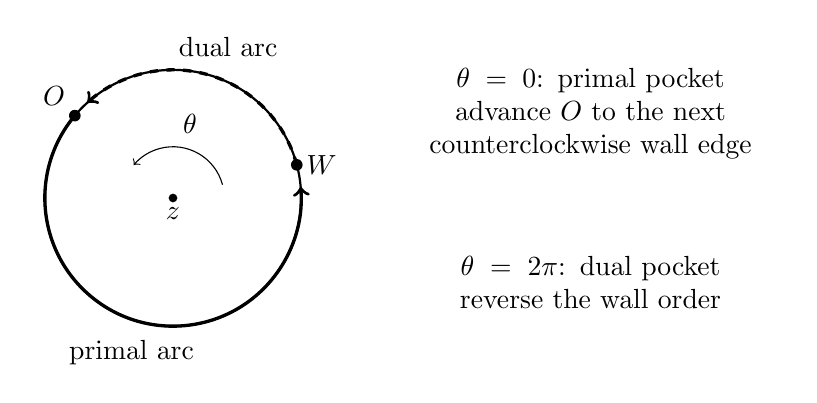
\begin{tikzpicture}[scale=1.05]
 \draw[thick] (0,0) circle (1.55);
 \draw[very thick,dashed,->] (15:1.55) arc (15:132:1.55);
 \draw[very thick,->] (140:1.55) arc (140:365:1.55);
 \fill (0,0) circle (1.5pt) node[below] {$z$};
 \fill (15:1.55) circle (2pt) node[right] {$W$};
 \fill (140:1.55) circle (2pt) node[above left] {$O$};
 \draw[->] (15:.62) arc (15:140:.62);
 \node at (77:.92) {$\theta$};
 \node at (70:1.95) {dual arc};
 \node at (255:1.94) {primal arc};
 \node[align=center,text width=4.8cm] at (5.05,1.02)
 {$\theta=0$: primal pocket\\
  advance $O$ to the next counterclockwise wall edge};
 \node[align=center,text width=4.8cm] at (5.05,-1.02)
 {$\theta=2\pi$: dual pocket\\
  reverse the wall order};
\end{tikzpicture}
\caption{Normalized chart of a two-change component.  The angle
$\theta=O-W$ is measured counterclockwise along the dual arc.
The arrows on the circle indicate boundary order, not strand
orientation.  The forcepoint reset uses the next old-wall edge on the
retained pocket.  A full turn changes the endpoint of the reflected
angular interval.  The drawing is schematic; microscopic tip and
force sides are suppressed.}
\label{tree:figure}
\end{figure}

Away from coincidences use Lemma~\ref{tree:interior}.  In an endpoint
zone, a fast exit toward the interior is controlled by the tightness
of $\theta$, and fast motion remaining in that zone is controlled by
Lemma~\ref{tree:bar} and the sign of $O$.  Thus $W$ and $O$ are
continuously tight, also at variable stops.  Moreover, on a sufficiently
small fixed endpoint zone, both the continuous part of $O$ and every
reset have the same sign.  Its variation on each visit is bounded by
its angular oscillation there.  Count visits by alternations between
nested endpoint zones, whose number is tight; outside these zones the
cotangent rate is bounded.  We obtain tightness of
\begin{equation}\label{tree:variation}
 \operatorname{Var}_{[0,T]}(O)
 \quad\hbox{and}\quad
 \int_0^T|\cot(\theta_t/2)|\,dt.
\end{equation}
In any limit the endpoint sets have zero radial Lebesgue measure,
$O$ has locally finite variation, and \eqref{peel:force-ode} holds off
those sets.  A remaining singular part could only be nonnegative at
$0$ and nonpositive at $2\pi$.  We next rule it out.

\subsection{Instantaneous reflection and removal of a singular push}
\label{tree:endpoints}

\begin{proposition}[The endpoint convention is determined]
\label{tree:reflection}
In its own radial clock, the limiting gap is the unique instantaneous
reflected diffusion on $[0,2\pi]$ with interior generator
\begin{equation}\label{tree:generator}
 \mathcal A f(\theta)=\frac\kappa2 f''(\theta)
       +\frac{\kappa-4}{2}\cot(\theta/2)f'(\theta).
\end{equation}
The forcepoint has no singular push:
\begin{equation}\label{tree:no-push}
 O_t=O_0+\int_0^t\cot(\theta_s/2)\,ds.
\end{equation}
Equation~\eqref{tree:sde} consequently holds globally, including
collisions, with locally integrable drift.
\end{proposition}

\begin{proof}
For a smooth function constant near both endpoints, the localized
interior identities glue to the martingale problem for
$\mathcal A$.  To admit a smooth function with
$f'(0)=f'(2\pi)=0$, approximate it by such cutoffs with uniformly
bounded second derivatives.  Its cotangent term is bounded near the
ends, since $|f'(\theta)|=O(\min(\theta,2\pi-\theta))$.
The endpoint time is zero, so dominated convergence gives the limiting
martingale identities and, by applying the same argument to $f^2$,
their brackets.

In particular $X=\cos(\theta/2)$ solves
\begin{equation}\label{tree:jacobi}
 dX_t=\frac{\sqrt\kappa}{2}\sqrt{1-X_t^2}\,dB_t
           -\frac{3\kappa-8}{8}X_t\,dt,
 \qquad -1\le X_t\le1.
\end{equation}
The diffusion coefficient is one-half H\"older and the drift is
Lipschitz; the one-dimensional square-root uniqueness criterion gives
pathwise uniqueness.  Hence this equation fixes the instantaneous
reflected law of $\theta$; a sticky alternative is also excluded by
zero endpoint time.

Near either endpoint the scaled distance $R$ has Bessel dimension
\begin{equation}\label{tree:bessel-dimension}
 \mathfrak d=3-\frac8\kappa\in(1,2).
\end{equation}
Its drift differs from $(\mathfrak d-1)/(2R)$ by a bounded smooth
term of order $R$.  Stopped Girsanov, equivalently in the squared
coordinate where the excess drift divided by the diffusion coefficient
extends boundedly, transfers the usual Bessel path properties.  Thus
$\theta$ is locally H\"older of every exponent below $1/2$, and each
endpoint set has Hausdorff dimension at most
\begin{equation}\label{tree:zero-dimension}
 d_0=1-\mathfrak d/2<1/2.
\end{equation}
The needed Bessel H\"older statement is, for example,
\citet[Theorem~1.2 and Corollary~2.14]{HutzenthalerJentzenNoll2014}.
The zero-set statement follows from the inverse-local-time description
in \citet[Exercise~XI.1.25]{RevuzYor1999} and the stable-range dimension
in \citet[Theorem~III.15]{Bertoin1996}.  Only a bounded stopped
perturbation at one endpoint is being used here.

Write the possible remaining term as the signed measure
\[
 d\nu=dO-\cot(\theta/2)\,dt.
\]
It is supported on the two endpoint sets and has the sign specified
after \eqref{tree:variation}.  We give the time-block argument
explicitly, so that a Hausdorff-dimension bound, rather than an unstated
Minkowski bound, suffices.  Choose $\eta>0$ so small that
\[
 p=\tfrac12-\eta>d_0,
 \qquad u_m=2^{-m},\qquad r_m=u_m^p.
\]
By the H\"older property, every sufficiently fine dyadic block of
length $u_m$ meeting an endpoint set has its end-gap at most $r_m/32$
throughout.  Indeed choose a H\"older exponent strictly between $p$
and $1/2$.  Apply Lemma~\ref{tree:bar} with harmless fixed buffer
changes to the finitely many blocks at level $m$, taking the mesh
limit first.  The probability that some level-$m$ block stays in the
stated endpoint zone and has one-signed $O$-variation exceeding $Cr_m$
is at most
\begin{equation}\label{tree:block-sum}
 C(1+T/u_m)\exp(-c u_m^{-\eta}).
\end{equation}
This is summable in $m$.  The estimate for $O$ follows from that for
$W$ because their difference is the end-gap, of size at most $r_m/32$
on such a block.  Borel--Cantelli gives, almost surely, the variation
bound $Cu_m^p$ on every sufficiently fine endpoint-meeting block,
separately for the two endpoints and on each fixed horizon.

On an endpoint neighborhood, $dO$ is one-signed, and so is the
cotangent time measure.  Its restriction to the endpoint set is zero,
whereas the restriction of $dO$ there is precisely $d\nu$.
Consequently $|\nu|(I)\le\operatorname{Var}_I(O)$ for every small
interval in that neighborhood.  Cover the endpoint set by intervals
of variable lengths whose sum of $p$th powers is arbitrarily small,
using \eqref{tree:zero-dimension}.  Replace each by a bounded number
of comparable dyadic intervals that meet the set.  The preceding
variation bound yields arbitrarily small $|\nu|$-mass.  Thus
$\nu=0$, proving \eqref{tree:no-push}.

Finally, a Bessel process of dimension greater than one is a
semimartingale with integrable inverse-distance drift and no local-time
term in its ordinary coordinate.  Undoing \eqref{tree:jacobi} in the
endpoint neighborhoods, and using the interior identities elsewhere,
gives
$d\theta=-\sqrt\kappa\,dB+((\kappa-4)/2)\cot(\theta/2)dt$.
Together with \eqref{tree:no-push} this is \eqref{tree:sde} globally.
There is therefore no unspecified boundary pushing rate.
\end{proof}

\subsection{Common clocks and independence after separation}
\label{tree:joint}

The single-branch conclusion does not by itself identify the joint
tree.  In particular a narrow discrete corridor may survive after its
two limiting target kernels have separated.  We address this before
using any continuum tree theorem.

\begin{proposition}[Joint target tree]\label{tree:joint-law}
For every finite family of deterministic interior targets, the peeling
converges in its joint radial driving data to the target-invariant
branching radial $\mathrm{SLE}_\kappa(\kappa-6)$ tree.  Branches agree
until their target kernels separate and then have independent
continuation noises.  At successive full turns the force side is
reversed, equivalently the angular gap remains instantaneously
reflected on $[0,2\pi]$.
\end{proposition}

\begin{proof}
Use the sum of currently accrued target clocks as a common parameter
$v$, freezing each target at its prescribed horizon.  Every clock
$t_i(v)$ is nondecreasing and $1$-Lipschitz.  Several run together while
their targets share an active component; separate components are
processed in serial priority order.  A flat clock has a constant state.
All tightness bounds and the interior identities hold between adapted
common-clock stops, including tests of the whole past.  Work in other
components during an interrupted segment is conditionally independent
of its unqueried switches by Lemma~\ref{peel:factorization}; neither
the schedule nor the stop gives advance information.

Extract limits jointly with the clocks.  The preceding endpoint
arguments can be applied in each marginal's own radial clock, using
tightness and inverse-clock extraction across flat stretches.  Thus
the martingale part $M_i$ of $W_i$ is a continuous local martingale
relative to the common past, with
\begin{equation}\label{tree:brackets}
 d\langle M_i\rangle=\kappa\,dt_i.
\end{equation}
The Loewner equations determine its target kernels and normalized
maps.

While targets $z_i,z_j$ remain in one component, put
$\xi=\Phi_i(z_j)$.  Radial Loewner evolution and the conformal-radius
change give
\begin{equation}\label{tree:clock-change}
 dt_j=P^2\,dt_i,\qquad
 d\log|\xi|=P\,dt_i,\qquad
 P=\frac{1-|\xi|^2}{|e^{iW_i}-\xi|^2}.
\end{equation}
Their marked boundary angles correspond by the normalized disk
M\"obius map.  On a compact interval with $|\xi|<1$ these formulas
are regular and pass to the limit.  The targets are still in the same
kernel exactly while they retain an interior connecting path: kernel
convergence preserves paths with positive clearance.  Thus they have
the same growth up to kernel separation.

Suppose now their limiting kernels have separated but their discrete
components have not yet split.  Along such a portion $|\xi|\to1$ by
monotonicity.  On a subinterval where both limiting angle gaps stay in
the interior, the two marked prepoints remain separated in both
charts.  The disk M\"obius formula forces one of
$e^{iW_i},e^{iO_i}$ to be within $C(1-|\xi|)$ of $\xi$ in the
prelimit.  Since they are separated in the $i$-chart, the choice cannot
change on a connected subinterval.  If it is the tip, $P\to\infty$;
if it is the forcepoint, $P\to0$.  Equation~\eqref{tree:clock-change}
then forces one limiting clock to be flat.  This remains true along
subsequences of exact discrete split times.  After an exact split,
serial growth gives disjoint time interiors for the two clocks.
There are only boundedly many changes of component choice for a finite
target list and finite horizons.  Endpoint angle sets have zero mass
for the corresponding own clock by Proposition~\ref{tree:reflection}.
The covariance inequality for continuous local martingales and
\eqref{tree:brackets} therefore show that
\begin{equation}\label{tree:orthogonal}
 d\langle M_i,M_j\rangle=0
 \quad\hbox{after their kernel separation}.
\end{equation}
Frozen targets are omitted from this comparison.

We spell out why these characteristics determine independent
continuations, without asserting that the clocks are independent.
In each still-accessible active group choose its first indexed target
as representative.  Until a separation or freeze, the representative's
motion determines all other states and clocks by
\eqref{tree:clock-change}.  Separation and freeze times are intrinsic
stopping stages: mutual accessibility is read from the radial ODE up
to first approach to unit modulus.  While two other members remain
regular with the representative, they cannot lose their shared access
before either is lost from that representative.  A nonrepresentative's
horizon is likewise read by its clock correspondence.  At a multiple
separation, take the continuous state limits in all own clocks; the
subgroups are exactly those retaining internal mutual paths in their
kernels.  Serial speeds of unrelated groups have no effect on these
stages.

For each target accumulate its martingale coordinate only over the
suffix during which it is an active representative, keeping it flat
otherwise.  More precisely, with the predictable choice at the stage
endpoints, set
\[
 N_i(v)=\int_0^v
 \mathbf 1_{\{i\text{ is an active representative at }s\}}\,dM_i(s).
\]
Once it becomes representative it remains representative of its
descendant group until it freezes.  These representative martingales
$N_i$ are pairwise orthogonal by \eqref{tree:orthogonal}.
Their terminal brackets can be finite, so make the completion explicit.
Let $T_i$ be the prescribed horizons and take the deterministic common
terminal parameter $V=\sum_iT_i$, extending all stopped states constantly
if necessary.  Divide each $N_i$ by $\sqrt\kappa$, and enlarge the
common filtration after $V$ with
independent Brownian motions $\widehat B_i$, independent also of the
entire original terminal sigma-field.  Set
\[
 \widehat N_i(V+s)=N_i(V)/\sqrt\kappa+\widehat B_i(s),\qquad s\ge0,
\]
and use $\widehat N_i(v)=N_i(v)/\sqrt\kappa$ for $v\le V$.
The extended processes are continuous local martingales in this
enlarged common filtration, remain pairwise orthogonal, and have
infinite terminal brackets.  Knight's orthogonal-martingale time-change
theorem now gives independent standard Brownian motions in their
respective bracket clocks
\citep[Theorem~V.1.9]{RevuzYor1999}; see also
\citet[Theorem~2]{Meyer1971Knight}.
Restricting to each original terminal bracket supplies precisely its
original representative martingale.  The auxiliary continuation changes
neither the past filtration nor any stage of the exploration.

For the conditional assertion, let $\mathcal G_v$ be the common causal
filtration and let $S$ be a separation or freeze stage.  Restart the
active representative martingales at $S$, stop at the next common stage,
and pad constantly to a deterministic horizon.  After localizing to
bounded brackets, these restarted processes remain orthogonal
martingales under $\mathbb P(\,\cdot\mid E)$ for every $E\in\mathcal G_S$ of
positive probability, with the same bracket identities.  Completing
them as above and applying Knight's theorem under this measure gives
the same product Wiener law for every $E$.  Thus the continuation
noises are independent of $\mathcal G_S$.  A continuing representative
uses its original martingale increments, and a newly selected one
starts its representative suffix.  No conditioning on terminal
bracket values or future separation data is involved.

The pathwise uniqueness of \eqref{tree:jacobi}, followed by
\eqref{tree:no-push}, determines the angles and maps through the next
intrinsic stage.  A newly assigned representative uses its assigned
independent noise; a continuing one uses the continuation of the same
Brownian solution.  A change caused solely by a representative's
horizon gives a fresh continuation at that stopping stage.  Induction
over the finite target groups identifies the usual common-branch,
independent-after-separation construction.

The resulting equations and angular convention are the target-invariant
radial tree of
\citet[Propositions~3.13--3.14 and Section~4.2]{Sheffield2009Exploration}:
a one-sided force weight $\kappa-6$, with the side reversed in an
enclosed component after a full turn.  Our sign convention is
$\theta=O-W$; exchanging the sign of its Brownian motion translates
to the opposite angular convention.  Increasing the finite horizons
proves the assertion at all finite clocks.
\end{proof}

\section{Recovery of the nested loop collection}
\label{sec:loops}

Continue first in a fixed axis-parallel square with the primal-open
wall and wired law of Subsection~\ref{peel:construction}.  Draw the two
pairs at each tile contact disjointly in a midpoint disk of radius
less than $\delta/100$, taking each turn on its prescribed side.
The resulting actual loops are simple, pairwise disjoint, and avoid
actual open diagonals of both colors.  Use the analogous drawing for
wall triangles and orient every loop primal-left.  Matching successive
traversal pieces inside those disks changes each loop by at most
$2\delta/100$ in Euclidean uniform curve distance, and by a constant
multiple of this in spherical distance, simultaneously for all loops.
Thus the drawing convention has no effect on the desired topology.

\subsection{Compactness and two sides of every limiting loop}
\label{loop:compactness}

\begin{lemma}[Positive-law loop geometry]\label{loop:geometry}
The closed loop collections in the fixed square are tight for matching
uniform curves modulo reparametrization and orientation.  Constant
limit curves may be removed.  Their positive-diameter subsequential
limits have the following properties almost surely.
\begin{enumerate}[label=\textup{(\roman*)}]
\item Each deterministic interior point lies on no loop.  Its absolute
winding number about any loop is $0$ or $1$, and is stable along a
converging loop sequence.
\item No interior point has three distinct visits in total among the
loop elements.  Visits include multiple traversals after constant
pauses are removed and also multiplicity of different elements.
\item At every interior point of a positive loop, every neighborhood
contains open disks of both absolute winding statuses for that loop.
\end{enumerate}
\end{lemma}

\begin{proof}
\textit{Passage counts and compactness.}
Consider a vertical band of fixed positive width, with its vertical
sides interior to the square and its height equal to that of the
square.  Each disjoint medial passage between its sides has an actual
dual path beside it: consecutive adjacent dual vertices are identical
or joined by an open dual diagonal, including at wall caps.  Crop to
a slightly narrower band.  The medial separators continue beyond both
cropped sides and are disjoint from dual-open edges, so they divide
the band into strips.  Each accompanying dual path lies in the strip
on its separator's dual side, with at most two assignments to a strip.
Paths in different such strips cannot communicate in the actual dual
graph there.  Hence many passages force many distinct actual dual
components crossing the cropped band.

The graph of internal dual faces is a full lattice rectangle with
arbitrary induced boundary data; it has no dual crossing of the
initial deterministic primal wall.  The disjoint-passage proof of
Lemma~\ref{peel:passages} bounds its crossing-component count.
Even with all boundary vertices wired, an \emph{actual} left-right
crossing is bounded away from probability one by an up-to-boundary
primal blocker.  End that blocker just beyond the extreme dual rows
by bounded finite-energy extensions to neighboring internal primal
vertices.  The rectangle's dual boundary edges themselves are random,
so the crossing theorem applies.  The same argument holds for
horizontal bands.

A finite family of trimmed bands at each fixed scale bounds both the
number of loops with diameter above that scale and the number of their
disjoint subarcs with a given positive displacement.  These bounds
yield compactness modulo reparametrization.  To make the extraction
explicit, subdivide each positive loop by successive first-displacement
times into arcs of diameter at most $2^{-j+O(1)}$, retaining marks from
previous subdivisions.  The number of marks at each fixed $j$ is
tight.  Pass to subsequences on which their positions and cyclic orders
converge.  Assign nested parameter intervals with maximal length
tending to zero and positive lengths at every fixed subdivision,
splitting an interval further in two when necessary.  The corresponding
polygonal curves approximate uniformly.  Diagonalize over diameter
cutoffs tending to zero, retaining multiplicities of matched elements.
This proves collection tightness.

\paragraph{Avoidance and the visit bound.}
For a deterministic interior point, RSW circuits in successive
concentric annuli obstruct an actual arm to a fixed positive distance.
The probability that a macroscopic loop approaches that point tends
to zero with the inner radius.  A countable union over diameter
cutoffs gives (i).  Winding is stable under uniform convergence away
from the point, and each simple discrete loop has absolute winding
$0$ or $1$.

Three distinct positive visits near an interior point would yield six
medial passages through arbitrarily small annuli out to a fixed
positive scale.  This includes visits belonging to different collection
elements.  In a trimmed intermediate annulus, order those radial
separators and assign their actual color arms to the intervening
strips.  Arms in distinct strips stay separated.  Where a strip
receives two assignments retain both if their colors differ, and one
if their colors agree.  Each separator marks a color transition, so
the resulting cyclic sequence has an alternating subfamily of at
least six arms.  Radial buffers justify all croppings.  The six-arm
bound of \citet[Corollary~6.7]{DMT2021Fractal}, transferred to this
positive square law through a bulk collar, has exponent $2+c$ for
some $c>0$.  A grid union over possible centers therefore vanishes
like a positive power of the inner scale.  Taking mesh limits first
proves (ii).

\paragraph{A circuit attached to each macroscopic bank.}
Fix a bulk core rectangle, with buffer space around it, and a color
$X$.  We claim that, with probability tending to one as $m\to\infty$
after the mesh limit, the actual cluster of every bottom-to-top core
crossing contains an $X$-open circuit in the buffered patch enclosing
a disk of radius $c/m$.

In a first subrectangle ending at a middle row, label the actual
connected components joining its two terminal rows.  Their number is
tight by the passage bound.  Reveal the past up to that middle row.
Above it use $m$ fresh transverse slabs of height $h\asymp1/m$,
with all levels rounded on the $X$-grid.  For a given label, its
sources are its actually connected bottom vertices.  At each new row
ask whether these sources connect to that row in the cumulative core
rectangle.  A full crossing survives all these tests under one of
the initial labels.

When a label survives to a row, choose the leftmost simple open path
from its sources to that row.  The edges strictly to its right are
fresh with domain Markov data.  Indeed attach auxiliary spokes from
one point below to the sources and from the new top row to a point
above, in a disk with these auxiliary endpoints on its boundary.
Simple paths use spokes only at their ends.  Minimizing left area
selects a path determined by its own edges and those on its left:
any path entering strictly left supplies an open excursion between
two distinct selected-path vertices that decreases the left region.
The ordinary lattice part $p$ is actually connected to the label.

At the slab's middle height, approach horizontally from the right
exterior of the core and choose $x$ on the right at distance $h/16$
from $p$.  The ball $B(x,h/3)$ lies in the wider fresh patch, far
from the past, spokes, and slab ends.  The fresh graph on the right
of $p$ inside a slightly buffered ball dominates the restriction of a
free comparison on the full ball graph.  All attachments from omitted
left-side or path edges go through vertices of $p$, which are wired
by actual connectivity in the conditioned law.  This argument applies
to either color, using the dual FK law for dual $X$.

By interior RSW and FKG in the free ball comparison, with probability
at least a fixed $c'>0$ there is an open circuit between radii
$h/64,h/24$, connected there to one between radii $h/8,h/4$.
The outer circuit meets the deterministic geometric path $p$, since
$p$ comes within $h/16$ of $x$ and exits the ball.  Both use the same
color graph.  The inner circuit is wholly on the right of $p$, as is
its connection up to first contact with $p$.  Therefore this event
supplies an actual attached disk-circuit using only fresh right-side
edges in the slab.  Conditionally on survival, failure to acquire such
an attachment costs a factor at most $1-c'$ at each stage.  Truncate
the initial number of labels and iterate.  This proves the claim.

\paragraph{Visibility of both winding statuses.}
Use countably many core tests with rational positions and buffered
sizes.  A varying portion of a limiting loop in an interior ball
crosses two horizontal or vertical levels of one such test with
clearance.  In its discrete approximants the two actual color banks
supply crossings.  Their clusters lie on opposite sides of the simple
loop and do not cross it.  Choose the buffered test much smaller than
the loop's diameter, so neither of the attached disk-circuits can
contain the entire loop.  The disks strictly inside the two circuits
then have the two corresponding winding statuses.  Shrink them to
retain positive clearance; subsequential limits preserve disks of
positive radius in the prescribed ball.  The preceding estimate makes
failure arbitrarily unlikely.  Every neighborhood of a point on a
nonconstant loop contains a varying portion, so the countable tests
prove (iii) simultaneously.
\end{proof}

\subsection{Canonical loops and their continuation in the tree}
\label{loop:canonical}

Take joint subsequential couplings of the loop collections and of the
angular trees for a countable dense set $\mathcal Z$ of deterministic
interior targets, with arbitrarily large finite clock horizons.
Lemma~\ref{loop:geometry}(i) ensures that all these targets avoid all
positive limiting loops almost surely.  Incidental lattice-edge
positions do not require an extra convention: each active finite
horizon retains a ball around its target.

We specify the established continuum input before making the lattice
identification.  For $4<\kappa<8$, the target-invariant tree of
\citet[Sections~4.2--4.3]{Sheffield2009Exploration} constructs the
surrounding loops by full-turn angular excursions and completes each
partially traced loop through the other branches.  At the time of
that paper, its stated continuity and invariance conclusion in
Proposition~5.1 was conditional.  Here the needed hypotheses follow
from \citet[Theorem~1.3]{MillerSheffield2016IG1} and
\citet[Theorem~1.2 and the ensuing CLE discussion]{MillerSheffield2016IG3}.
For our single one-sided force weight, $\kappa-6>-2$, so force
collisions do not reach the continuation threshold.  For reversal,
the two one-sided weights $\kappa-6$ and $0$ are both at least
$\kappa/2-4$.  The starting square is a Jordan domain, and all
specified targets are distinct interior points off the loops.  These
results supply continuous non-simple CLE loops and their conformal
and anticonformal invariance under exactly the parameters used here.
They assert no lattice convergence or traversal identification.

The tree in Proposition~\ref{tree:joint-law} therefore has a coupled
canonical nested $\mathrm{CLE}_\kappa$ collection in the square.
Starting from a primal wall, let $b_0=0$, and let $b_1,b_2,\ldots$
be the successive hits of the alternating opposite endpoints:
first $2\pi$, then $0$, and so on.  Let $a_k$ be the last visit to
the starting endpoint before $b_k$.  The canonical surrounding loop
is denoted $\widetilde L_z^k$.  It follows the branch toward $z$ on
$(a_k,b_k)$ and is then completed to its starting point by the tree's
continuation of the current strand.  These are the successive loops
with nonzero winding about $z$, and every canonical loop is obtained
from a target in $\mathcal Z$.

The endpoint reversal amounts to using reflected exploration chirality
in the new enclosed component.  Nesting supplies independent CLEs in
those components, and anticonformal invariance preserves their
unoriented laws.  Thus the alternating endpoint convention gives the
same nested ensemble.  The scalar full-turn description is also the
one in \citet[Proposition~2]{SchrammSheffieldWilson2009}; that result
identifies the conformal-radius decrement, while the joint branch
coupling and loop completion used here come from the exploration-tree
construction.  Endpoint accessibility of the diffusion with
$1<\mathfrak d<2$ makes every $b_k$ finite, and $b_k\to\infty$:
otherwise its continuous angle would make infinitely many full
$2\pi$ swings on a compact clock interval.

We will need the following concrete interpretation of the completion.

\begin{lemma}[Default continuation and local double visits]
\label{loop:continuation}
At an interior-angle time $s\in(a_k,b_k)$, the remaining traversal
of $\widetilde L_z^k$ is the default strand from $W_s$ to $O_s$ in
the current domain.  In a chart sending those accesses to $0,\infty$,
every finite portion of this continuation is ordinary chordal
$\mathrm{SLE}_\kappa$ and is recorded by branches to targets from
$\mathcal Z$ that remain accessible high above that portion.
Every open nonconstant traversal interval of $\widetilde L_z^k$
contains two visits to one square-interior point.
\end{lemma}

\begin{proof}
The stopped chordal equivalence is only valid while its force access
is available.  To continue after the original target is cut off, use
the branch that retains this access, as prescribed by the tree
construction.  A bounded finite chordal-capacity portion has bounded
hull and driver.  An open set of targets mapped to sufficiently large
heights remains accessible above it, with tip and force angles strictly
separated on that portion.  The countable dense set supplies such a
target.  Its branch records the default continuation even if it has
already separated from $z$.  Target invariance gives consistency when
the target or the finite portion is enlarged.  This realizes all
finite portions and hence the complete strand; it does not extend
Proposition~3.12 of \citet{Sheffield2009Exploration} beyond its stopping
condition.

All these curves are continuous.  Over a finite trace time the
remaining domains have locally connected boundaries, by the
locally-connected-continuum boundary theorem applied to the continuous
trace and the starting boundary.  Their prime-access conformal images
can thus be regarded as continuous physical curves.

For ordinary chordal SLE, \citet[Theorem~1.1 and Corollary~1.7]{MillerWu2017}
give double points in the interior when $4<\kappa<8$.  Indeed their
double-point dimension exceeds the boundary-hit dimension by
$(\kappa-4)^2/(8\kappa)>0$.  Both visits occur at finite times.
Scaling makes the probability of such a double visit before time $t$
independent of $t>0$; since its union over finite times has probability
one, this probability is one for every $t>0$.  The domain Markov
property then gives an interior double visit in every rational open
capacity interval.  Conformal maps preserve an interior double visit.
Every open traversal interval of the canonical loop contains an
interior-time portion either of its full-turn excursion or of its
finite default continuation.  On a sufficiently short localized
portion its law is ordinary chordal SLE.  The preceding arbitrary-short-time
statement applies before any positive localization time,
proving the assertion.
\end{proof}

\subsection{Episodes and full-turn labels}
\label{loop:episodes}

A discrete \emph{episode} starts when a cap is opened and ends at the
next switch retaining a homogeneous pocket.  Its color is the
homogeneous wall color just before the opening.  Call it successful
when its loop winds around the target.

\begin{lemma}[Discrete winding order]\label{loop:episode-order}
As long as the target is macroscopically separated from a consumed
tile or star, an episode is successful exactly when its terminal
switch changes wall polarity.  These polarity changes enumerate all
loops surrounding the target, in their order from outside inward.
A positive loop with positive clearance from the target is reached
before a finite radial horizon depending on that clearance.
Conversely a successful switch by a bounded horizon has macroscopic
clearance from the target.
\end{lemma}

\begin{proof}
The loop through the newly opened cap lies inside its homogeneous
starting pocket.  At the cap, the side toward the base, of the
starting color, is exterior to this loop; the other side is interior.
During the episode the actual color banks preserve connections to
these sides.  If a bank hits its same-color wall, the retained
homogeneous target pocket is connected to the cap along that bank.
The traversed loop is outside the pocket: its past pairs have been
removed, the new open diagonal is a barrier, and the continuation to
the old force side stays in the main component.  The target can reach
that pocket's wall color without crossing the loop.  Comparing this
color with the starting color proves that the target is inside the
loop precisely at a polarity change.  The same argument works with
separate boundary occurrences.

Every other unstarted candidate surrounding the target stays intact
in the retained component.  Actual diagonals and walls cannot cross
it, and a loop wholly inside a simply connected pocket has its
interior there too.  Its deterministic pairs in any wall triangles
are also intact, because cuts by other loops never traverse them.
If the loop entered at a new cap surrounds the target, it is outermost
among the remaining candidates: its access to the homogeneous wall
at that cap crosses none of them.  Thus successful episodes enumerate
the surrounding loops, with possible unsuccessful same-color episodes
between them.

Before such a loop's episode, growth remains outside its enclosed
region; during the episode it follows that loop up to step-sized
errors.  A ball centered at the target inside its region therefore
survives until the switch.  If its radius is $r>0$, then
$\operatorname{crad}(U_t,z)\ge r$ up to that time, bounding the
radial clock by $\log(\operatorname{crad}(U_0,z)/r)$.
Conversely, Koebe's bound on a fixed horizon gives a positive-radius
ball in the newly retained pocket, and its surrounding successful
loop lies outside that ball, up to vanishing step errors.
\end{proof}

An endpoint approach could otherwise be mistaken for a reset in the
limit.  The next estimate excludes this possibility.

\begin{lemma}[Endpoint resets cannot be skipped]
\label{loop:no-skip}
At a bounded-clock completed state with $\theta$ approaching $0$,
the probability of returning to a fixed positive angle before a
primal-pocket reset tends to zero, with the mesh limit first and the
endpoint tolerance second.  The analogous assertion near $2\pi$
uses a dual-pocket reset.  Consequently the true successive discrete
polarity-change times $b_k^n$ converge in probability to $b_k$ on
sufficiently large finite horizons.

Moreover, in an episode that succeeds by a bounded horizon, after a
fixed interior-angle advance the probability of retreating arbitrarily
near its starting endpoint before its successful switch tends to zero
in the same order of limits.
\end{lemma}

\begin{proof}
Near $0$ the entire dual wall arc and both end sides are in a tiny
boundary neighborhood of the stopping chart.  Until a primal reset,
the growing dual bank remains actually connected to that arc; stop
also before a fixed interior-angle threshold, so no opposite-end
switch has yet occurred.  In successive buffered dyadic chart
half-annuli around this neighborhood, place actual primal transversal
paths from primal wall to primal wall.  Lemma~\ref{peel:wall-rsw}
gives a uniformly positive conditional success chance at each
separated scale, after the mesh limit at the chosen cutoffs.  A
successful path confines the connected dual bank, and hence the slit
pieces, inside its small wall sector.

A hull confined to such a sector has a small new angular footprint:
its basepoint-side maps converge to the identity at the origin and,
by reflection, on each closed boundary arc away from that sector.
The trapped dual arc remains in its short footprint.  Therefore it
cannot produce a fixed positive angular advance.  Letting the number
of half-annuli grow proves the first assertion.  Exchange colors and
reverse directions at $2\pi$.

A true polarity change approaches the specified opposite endpoint,
up to vanishing update errors.  Uniform angle convergence and induction
therefore preclude a premature macroscopic limit for $b_k^n$.
Conversely, after the limiting first endpoint hit, instantaneous
reflection produces a positive excursion within any prescribed
additional time almost surely.  Truncate the clocks and choose an
exit size so that failure has arbitrarily small probability.  Start
at the first completed-state approach within a small tolerance after
the previous true polarity change.  The just-proved estimate excludes
an excursion of this size before the corresponding reset.  Let the
tolerance tend to zero.  An earlier matching reset already suffices.
Thus no endpoint hit is skipped, and $b_k^n\to b_k$.

For the final assertion, stop at successive approaches to the starting
endpoint after a fixed-size advance.  A successful episode that makes
such an approach must then advance macroscopically without the
corresponding same-color reset, since that reset would end the episode.
The first assertion bounds each such event.  The number of fixed-size
swing tests is tight by angular tightness, so truncation and iteration
give the stated retreat estimate.
\end{proof}

It follows in particular that on every compact subinterval of
$(a_k,b_k)$, the prelimit target branch is, with probability tending
to one, in the same episode as at its $k$th successful switch.  The
angle stays away from the starting endpoint on that compact interval,
and the preceding polarity change occurs before it.

Include the true winding-loop labels $L_z^{n,k}$ in the coupling and
extract their limits $L_z^k$, increasing clock and diameter cutoffs
as needed.  They have positive size at bounded $b_k^n$ by
Lemma~\ref{loop:episode-order}.  They exhaust the positive limiting
loops winding about $z$: any such loop has positive clearance from
$z$ and is reached before a bounded horizon, while the number of full
swings there is tight.  Winding tests are stable.  For finite lists of
labels stabilize also the indicators of equality as collection
elements and then diagonalize.  Distinct elements in this bookkeeping
have distinct discrete representatives, even if their geometric limits
might initially appear identical.

\subsection{Ordered containment and equality of the labels}
\label{loop:matching}

\begin{lemma}[The canonical traversal is contained in order]
\label{loop:ordered}
For each $z\in\mathcal Z$ and $k\ge1$, the entire traversal of
$\widetilde L_z^k$ occurs in cyclic order in $L_z^k$, possibly with
extra traversal portions inserted.  Its order occupies at most one
turn of $L_z^k$.  If two canonical labels give the same element, their
lattice-limit labels give the same collection element.
\end{lemma}

\begin{proof}
Fix a rational $s\in(a_k,b_k)$.  In any open subinterval of
$(a_k,s)$ choose $t<t'$ strictly inside it.  The target kernel strictly
shrinks between these times.  There is a new boundary point inside
the earlier open kernel; it belongs to the continuous canonical trace
over $[t,t']$.  Every small ball about this point with closure in the
earlier kernel must encounter new prelimit growth between the
corresponding times.  Otherwise the ball stays clear of new boundary.
It also meets a compact internal patch of the later kernel.  Connectedness
then puts that whole ball in the retained prelimit component, extending
the limiting kernel through its alleged boundary point, a contradiction.
These prelimit boundary pieces are slit updates tracing the successful
episode, up to vanishing physical step errors.

Apply this test simultaneously to any finite ordered list of such
intervals.  Completed-update stops can be moved slightly inside them
because capacities and angular within-step errors vanish.  We obtain
points of the discrete winding-loop traversal, in chronological order,
converging to canonical trace points in those intervals.

Now take any finite list of finite chordal intervals on the default
continuation after $s$.  Choose, realization by realization, a target
$w\in\mathcal Z$ in the current kernel whose chart image is safely
above the entire bounded portion in question.  It was still accessible
with $z$ up to $s$.  Their time correspondence there is regular and
passes to the mesh; they cannot have split earlier because the limiting
kernel contains internal connecting paths with clearance.  The branch
toward $w$ follows the default continuation with tip and force angles
separated by a positive margin on the selected portion, by
Lemma~\ref{loop:continuation}.  Therefore its discrete branch has no
reset there and continues the same original winding loop, in order,
after the common prefix.  The new-boundary test applies to these
intervals in the $w$-clock.  The target $w$ need not have a successful
episode for this loop.  Its post hoc choice costs no uniformity
assumption: all targets, clocks, and regular sharing correspondences
from the countable set have already been included in the coupling.

By continuity, shrinking the testing intervals and increasing the
finite continuation range shows that every finite increasing list of
canonical traversal points has representatives in order on $L_z^k$.
On a countable dense set of canonical parameter values, take a
single nondecreasing cyclic choice of representative parameters by
compactness and a diagonal subsequence.  Omitted endpoint values are
included by continuity.  The order uses at most one turn: the discrete
episode and its no-reset continuation traverse a simple closed loop
from its released cap without passing that cap a second time.
Two separated canonical visits cannot collapse to one representative
parameter, because every intervening open traversal interval has
actual variation.

If $\widetilde L_z^k=\widetilde L_w^j$ but the two lattice-limit
elements were distinct, each would contain the same canonical
interior double visit from Lemma~\ref{loop:continuation}.  This would
give more than two total limiting visits at that point, contrary to
Lemma~\ref{loop:geometry}(ii).  Thus equal canonical labels have equal
lattice-limit labels, with multiplicity understood as stipulated above.
\end{proof}

The converse is essential: ordered containment alone would permit
several canonical labels inside one discrete limiting element.

\begin{lemma}[The converse label identification]
\label{loop:label-equivalence}
Almost surely, simultaneously for all $z,w\in\mathcal Z$ and
$k,j\ge1$,
\begin{equation}\label{loop:label-iff}
 L_z^k=L_w^j
 \quad\Longleftrightarrow\quad
 \widetilde L_z^k=\widetilde L_w^j
\end{equation}
as collection elements.
\end{lemma}

\begin{proof}
Only the forward implication remains.  On the event that the discrete
labels are shared, the two branches cannot split before entering this
common loop: before its episode the loop and its interior remain
intact across every cut by other loops.  Choose clock horizons large
enough to include both successful switches except on an arbitrarily
small event.

While they share a domain, write $\xi=\Phi_z(w)$.  For a fixed small
$e>0$, stop at first approach to $|\xi|\ge1-e$, if it occurs before
the relevant winding switches.  For fine mesh this can be a completed
state also satisfying $|\xi|\le1-e/2$.  An exact split cannot precede
this threshold inside the comparison range: the ODE and clock change
are regular for $|\xi|\le1-e/2$, and elementary capacities vanish
there.

We first show that an \emph{unstarted} loop surrounding both targets
at this stop has probability tending to zero as $e\downarrow0$.
Place separated dyadic chart half-annuli around the boundary direction
of $\xi$, between radius a multiple of $e$ and a fixed small radius.
Choose their buffered wall intervals to avoid the two marked accesses
and sides; deleting the bounded number of affected scales leaves a
number tending to infinity.  Each bar separates a sector containing
the radial access from $w$ to the wall from the sector containing $z$
and a remote wall portion.

Use an actual-color transversal path in each bar, choosing the color
to match one wall end.  At that end it reaches an actual wall vertex.
At the other it does so as well if the wall has the same color.  If
that wall has the other color, complete the path from its specified-color
triangle corner to the base by the segment of
Lemma~\ref{peel:wall-rsw}.  After trimming at first wall contacts this
is a simple crosscut in the prime closure.  Its added segment meets
only the one local cap pair, once.

An unstarted simple loop inside the domain surrounding both targets
must cross this screen at least twice: it must meet both of the
separated sectors, and its interior contains both targets.  It cannot
cross the actual open path, and cannot traverse that one cap pair
twice.  Thus one successful screen precludes the event, even with
mixed wall colors.  The conditional success probability of each
fixed-aspect buffered bar is bounded below by
Lemma~\ref{peel:wall-rsw}.  Iteration, with the mesh limit first,
proves the asserted small probability.

We next obtain a shared interior precursor for a shared successful
loop.  If the common loop is processed before the near-separation
threshold is needed, its episode visibly passes through interior
angles, comparable in the two charts while $|\xi|\le1-e/2$.
If the loop is still current at the threshold, its $z$-angle cannot
be arbitrarily close to that episode's starting endpoint and later
succeed without a same-color reset, by Lemma~\ref{loop:no-skip}.
Otherwise, its progression from the start to the current state has
already passed a fixed interior margin.  The $w$-angle at that shared
state has a comparable interior margin, with constants allowed to
depend on $e$.  The unstarted case has just been made unlikely.
Thus, except on an arbitrarily small event, the two successful
episodes have a common state before kernel separation, with both
angles interior by fixed positive margins.

From this precursor to the respective winding switches, neither angle
returns arbitrarily near its episode's starting endpoint, by the
successful-episode retreat estimate in Lemma~\ref{loop:no-skip}.
Choose in order the clock cutoff, the near-separation threshold, the
interior margins, and the retreat tolerance, making their error
probabilities successively small.  With strict buffers a subsequential
precursor remains in a common kernel with $|\xi|\le1-e/2$, lies after
both previous polarity changes, and lies in the interiors of both
limiting successful excursions.  Their endpoint histories and starting
excursion time agree along the common branch by the regular chart
correspondence.  They share the successful front to this interior
state and use the same default continuation to the same force access
for its rest.  Therefore their canonical loop elements coincide.
Let all the preceding errors tend to zero.  Countability of the
labels proves the simultaneous assertion.
\end{proof}

\subsection{Trace and traversal identification}
\label{loop:traversals}

\begin{proposition}[Identification away from the square wall]
\label{loop:identification}
Every positive lattice-limit loop with an interior point has a
canonical label.  Matched elements have the same winding indicators
on $\mathcal Z$.  If either matched element stays away from the square
wall, the two elements are equal as curves modulo reparametrization
and orientation.  Without that restriction, every canonical element
is still contained in order in its lattice-limit partner.
\end{proposition}

\begin{proof}
The two-winding-disk property of Lemma~\ref{loop:geometry}(iii)
provides a disk of winding one for every positive limiting loop with
an interior point.  It contains a target from $\mathcal Z$, so the
loop is one of its exhausted winding labels.  For a labeled loop,
Lemma~\ref{loop:label-equivalence} makes its dense-target winding
indicators identical to those of its canonical partner: winding one
at a target is equivalent to equality with one of that target's
successive surrounding-loop labels, in both collections.

Suppose an interior trace point of the lattice-limit loop were outside
its canonical partner trace.  A small ball about it avoids that
canonical trace and has constant canonical winding.  The two-winding-disk
property supplies disks of both lattice winding statuses in the
same ball, each containing a dense target.  This contradicts the
indicator equality.  Hence the entire interior lattice trace lies
on its partner.  The reverse trace inclusion follows from ordered
containment.  If the canonical partner is internal, the connected
lattice trace containing it cannot reach the wall without adding an
interior point outside that partner.  If the lattice trace is internal,
so is the contained partner.  Thus in either wall-away case the full
traces are equal.

It remains to exclude extra traversal of this trace.  Invert the
nondecreasing cyclic representative selection in
Lemma~\ref{loop:ordered} by a generalized inverse.  Because every
canonical open traversal interval has actual variation, this inverse
is continuous, nondecreasing, and of degree one.  The traces agree at
all its non-plateau-interior times.  A plateau would insert an extra
portion of the lattice traversal anchored at one canonical point.

Assume such a portion varies.  By trace equality it lies on the
canonical trace.  At a visited value different from its anchor there
can be only one canonical parameter: two canonical visits plus this
inserted visit would violate the total-visit bound of
Lemma~\ref{loop:geometry}(ii).  On a varying subarc away from the
anchor, the assignment to that unique canonical parameter is
continuous, by compactness.  It therefore sweeps a nontrivial canonical
traversal interval all of whose values have unique canonical visits.
This is impossible by the interior-double-visit property of
Lemma~\ref{loop:continuation}.  Hence every inserted portion is
constant.  Equality modulo reparametrization follows, including the
preserved multiplicity of collection elements.
\end{proof}

\subsection{From squares to the free plane law and the sphere}
\label{loop:wholeplane}

\begin{theorem}[Nested full-plane convergence for $q<4$]
\label{loop:plane}
For every fixed $1\le q<4$, the loop collection of the free
infinite-volume critical square-lattice FK law converges, through the
full mesh sequence, to the nested whole-plane
$\mathrm{CLE}_{\kappa(q)}$ in the spherical loop-matching topology
of Subsection~\ref{intro:collections}.  The limit is M\"obius invariant and includes every
nested generation.
\end{theorem}

\begin{proof}
We first give the uniform comparison estimates that allow an upgrade
from a local limit.  For a fixed compact disk $K$, the probability
that any discrete loop visits $K$ and reaches a distant surrounding
circle tends to zero as that circle tends to infinity, uniformly for
sufficiently small meshes and for larger initial wired squares.
Actual monochromatic circuits in buffered annuli block such a loop;
conditional RSW gives a fixed success chance at each separated scale.
Use a slightly enlarged $K$ and strict radial margins when passing
to limits.

The free infinite-volume law and the homogeneous-square law can be
coupled identically on a growing intermediate disk with probability
tending to one as the square grows.  Bracket the exterior partition
by the minimal and maximal partitions, use monotone FK coupling, and
expose actual boundary-attachment clusters in the maximal sample.
Dual RSW screens make their probability of reaching the deep interior
tend to zero.  Once exterior influence is separated, the remaining
conditional laws agree and one uses identical switches.  Combining
this with the preceding escape estimate makes the \emph{entire}
loops visiting $K$ coincide, since those loops stay in the intermediate
disk.  This argument uses the specified free plane law and FK domain
Markov coupling; it assumes no interface limit.

In a fixed-square subsequential coupling,
Proposition~\ref{loop:identification} identifies all wall-away
macroscopic loop elements, with their traversals.  Its remaining
possible discrepancies involve the wall.  The escape estimate makes
it unlikely that a lattice-limit loop both hits $K$ and reaches that
wall.  The same holds for a canonical CLE loop, because that loop is
contained in its lattice-limit partner.  Thus, when the square is
large, the square CLE and the free plane lattice law have arbitrarily
close matching configurations on loops visiting $K$, in the
successive mesh and square limits.

The large-domain local limit of nested CLE is established in
\citet[Appendix~A, Theorem~A.1]{MillerWatsonWilson2015}.  Its comparison
uses conformal identifications of the relevant random-region loop
configurations, with maps approaching the identity on compact sets;
it does not assert equality at unchanged Euclidean coordinates.
The work cited here is \emph{The conformal loop ensemble nesting
field}, arXiv:1401.0218, whose Appendix~A contains that theorem.
For $4<\kappa<8$ this construction agrees with the whole-plane
branching construction by
\citet[Remark~2.6]{GwynneMillerQian2021}, and its law is invariant
under inversion, hence under M\"obius maps, by their Theorem~1.1.
Centered squares and disks give the same local limit: normalize their
conformal radii, and the comparison maps tend to the identity on
compact subsets.  All these parameter restrictions hold for our
$4<\kappa\le6$.

To pass from this local law to the required spherical topology, fix
$\epsilon>0$ and choose $K$ so large that its exterior has spherical
diameter less than $\epsilon$.  Loops entirely outside $K$ are then
irrelevant at that matching accuracy.  The uniform escape bounds
control the loops that visit $K$ but leave a much larger disk.  They
hold for square CLEs uniformly as the squares grow, by their
subsequential square-law couplings and the containment argument above.
Consequently the laws of the square CLEs are Cauchy for spherical
matchings: compare two large squares on a large fixed intermediate
disk to the same free-plane lattice law, let the mesh tend to zero,
and use the escape tails and the exterior diameter bound.

Any resulting spherical limit has the established local whole-plane
CLE law.  That local law, together with these tails, determines the
full spherical collection: at each accuracy all relevant loops are
seen in a bounded window except on an arbitrarily small event.
Conversely, the same comparisons force every subsequence of the
free-plane lattice laws to this limit.  Hence convergence holds for
the full mesh sequence.  The target labels ranged over all $k\ge1$
and the clock cutoffs increased without bound, so no nested generations
have been discarded.  This proves Theorem~\ref{intro:main}(ii) for $1\le q<4$.
\end{proof}
